%!TeX program=xelatex
\documentclass[11pt]{book}

\usepackage{caption}
\usepackage[palatino]{anuthesis}
\usepackage{graphicx}
\usepackage{thesis}
\usepackage{makeidx}
\usepackage{xcolor}
\usepackage{hyperref}
\usepackage{amsmath}
\usepackage{amssymb}
\usepackage[numbers]{natbib}
\usepackage{wrapfig}
\usepackage[usenames,dvipsnames]{pstricks}
\usepackage[algoruled]{algorithm2e}
\usepackage{subcaption}
\usepackage{tikz}

\usepackage[T1]{fontenc}
\usepackage{fontspec}
\usepackage{xparse}
% The Palatino package gives a pretty terrible look to the PDF when compiling on
% Windows, so we need to use fontspec instead. Palatino Linotype exists on
% Windows but not on Mac (where Palatino exists instead). So...
\suppressfontnotfounderror1
\def\myfont{Palatino}
\def\myfallback{Palatino Linotype}
\count255=\interactionmode
\batchmode
\font\foo="\myfont"\space at 10pt
\ifx\foo\nullfont
  \font\foo = "\myfallback"\space at 10pt
  \ifx\foo\nullfont
    \errorstopmode
    \errmessage{no suitable font found}
  \else
    \let\myfont=\myfallback
  \fi
\fi
\interactionmode=\count255
\setmainfont{\myfont}

\usetikzlibrary{arrows}

% hyperref setup taken from Aladair Tran's thesis:
% github.com/chengsoonong/mclass-sky
\hypersetup{
    bookmarksnumbered,
    colorlinks   = true,
    urlcolor     = {blue!80!black},
    linkcolor    = {red!50!black},
    citecolor    = {blue!50!black},
}

\SetKwProg{WithProb}{with probability}{ do}{}

%%%%%%%%%%%%%%%%%%%%%%%%%%%%%%%%%%%%%%%%%%%%%%%%%%%%%%%%%%%%%%%%%%%%%%%
%% Preamble.

\title{Learning from Crowd Labels\\ to find Black Holes}
\author{Matthew Alger}
\date{\today}

\renewcommand{\thepage}{\roman{page}}

\makeindex
\begin{document}

%%%%%%%%%%%%%%%%%%%%%%%%%%%%%%%%%%%%%%%%%%%%%%%%%%%%%%%%%%%%%%%%%%%%%%%
%% Title page.

\pagestyle{empty}
\thispagestyle{empty}
%% Template titlepage.tex
%%
%% anuthesis.sty Copyright (C) 1996, 1997 Steve Blackburn
%%
%% Department of Computer Science, Australian National University
%%

\begin{titlepage}
  \enlargethispage{2cm}
  \begin{center}
    \makeatletter
    \Huge\textbf{\@title} \\[.4cm]
    \Huge\textbf{\thesisqualifier} \\[2.5cm]
    \huge\textbf{\@author} \\[8.5cm]
    \makeatother
    \Large A thesis submitted in partial fulfillment of the degree of \\
    \LARGE Bachelor of Science (Advanced) (Honours) at \\
    The Research School of Computer Science\\
    The Australian National University \\[2cm]
    \thismonth
  \end{center}
\end{titlepage}

%%% Local Variables: 
%%% mode: latex
%%% TeX-master: "thesis"
%%% End: 


%%%%%%%%%%%%%%%%%%%%%%%%%%%%%%%%%%%%%%%%%%%%%%%%%%%%%%%%%%%%%%%%%%%%%%%
%% Preliminaries.

%%
%% Template frontmatter.tex (Copyright etc.)
%%

\vspace*{14cm}
\begin{center}
  \makeatletter
  \copyright\ \@author
  \makeatother
\end{center}
% \noindent
% \begin{center}
%   \aboutthesis
% \end{center}
\noindent

\newpage

\vspace*{7cm}
\begin{center}
  Except where otherwise indicated, this thesis is my own original
  work.
\end{center}

\vspace*{4cm}

\hspace{8cm}\makeatletter\@author\makeatother\par
\hspace{8cm}\today


%%% Local Variables: 
%%% mode: latex
%%% TeX-master: "thesis"
%%% End: 


% % Dedication.

% \cleardoublepage
% \pagestyle{empty}
% %%
%% Template dedication.tex
%%

\vspace*{7cm}
\begin{center}
    To Palatino Linotype, a great font.
\end{center}


%%% Local Variables: 
%%% mode: latex
%%% TeX-master: "thesis"
%%% End: 



% Acknowledgements.

\cleardoublepage
\pagestyle{empty}
%%
%% Template ack.tex
%%

\chapter*{Acknowledgements}
\label{cha:ack}
\addcontentsline{toc}{chapter}{Acknowledgements}

    I would like to thank my lucky stars, and the cat, for not eating me.\\
    \begin{flushright}--- ANU Physics Thesis Template\end{flushright}

%%% Local Variables: 
%%% mode: latex
%%% TeX-master: "thesis"
%%% End: 



%%%%%%%%%%%%%%%%%%%%%%%%%%%%%%%%%%%%%%%%%%%%%%%%%%%%%%%%%%%%%%%%%%%%%%%
%% Abstract.

\cleardoublepage
\pagestyle{headings}
%%
%% Template abstract.tex
%%

\chapter*{Abstract}
\label{cha:abstract}
\addcontentsline{toc}{chapter}{Abstract}

This should be the abstract to your thesis\dots

%%% Local Variables: 
%%% mode: latex
%%% TeX-master: "thesis"
%%% End: 


%%%%%%%%%%%%%%%%%%%%%%%%%%%%%%%%%%%%%%%%%%%%%%%%%%%%%%%%%%%%%%%%%%%%%%%
%% Table of contents.

\cleardoublepage
\pagestyle{headings}
\markboth{Contents}{Contents}
\tableofcontents

%%%%%%%%%%%%%%%%%%%%%%%%%%%%%%%%%%%%%%%%%%%%%%%%%%%%%%%%%%%%%%%%%%%%%%
%% Main text.

\mainmatter

%% Chapters
% %!TEX root=thesis.tex
% Unsorted writing.

\chapter{Imagine There's No Chapters}
\label{cha:imagine}

\section{Papers Read}
\label{sec:papers}
  
  \begin{itemize}
    \item \citet{banfield15}
    \item \citet{yan10}
    \item \citet{yan11}
    \item \citet{dasgupta11}
    \item \citet{mozafari12} (re-reading in progress)
    \item \citet{fan15} (probably need to re-read)
    \item \citet{freund97} (need to re-read)
  \end{itemize}

\section{The Radio Galaxy Zoo}
\label{sec:rgz}

    Many galaxies contain a supermassive black hole in their centre. These
    black holes draw in surrounding matter, and may produce jets of matter as
    they do. These jets emit radio waves \todo{Or X-rays, I think, which are
    then redshifted to radio. Confirm and rewrite.} which can then be detected
    by radio telescopes. As black holes cannot be observed directly, this is
    the only way to identify black holes in distant galaxies. A radio-loud
    black hole in the centre of a galaxy is called an active galactic nucleus
    (AGN). \todo{I'm having some trouble finding information on AGNs,
    especially on their definitions. Find something concrete.} Large radio
    surveys such as Faint Images of the Radio Sky at Twenty-Centimeters (FIRST)
    \citep{white97, becker95} and the Australian Telescope Large Area Survey
    (ATLAS) \citep{franzen15} have found many sources of radio emissions, and
    these sources are dominated by AGNs \citep{banfield15}.

\section{Radio Galaxy Zoo Consensus Labels}

\section{Radio Cross-identification}
\label{sec:cross-identification}

    Each radio object has some associated infrared object called the host
    galaxy. The cross-identification task is to find the host galaxy given the
    radio object.
    
    For modelling the distribution, I have chosen to use logistic regression,
    i.e.
    \begin{equation}
        \label{eq:logistic-regression-cross-identification}
        p(y(x) = 1 \mid x, r) = \vec w \cdot \vec \phi(x, r)
    \end{equation}
    where $\vec \phi$ is a feature space mapping dependent on a galaxy and a
    radio object. The features should represent the galaxy in some way, so I
    have chosen the following feature space:
    \begin{equation}
        \label{eq:galaxy-features}
        \vec \phi(x, r) = \begin{pmatrix}
            \vec{\mbox{flux}}(x)\\
            \mbox{dist}(x, r)\\
            \vec{\mbox{cnn}}(\mbox{radio}(x))
        \end{pmatrix}
    \end{equation}
    $\vec{\mbox{flux}}(x)$ is a vector of infrared flux measurements of $x$,
    which can be obtained from the infrared survey catalogue. $\mbox{dist}(x,
    r)$ is the Euclidean distance across the sky between the centre of the $x$
    and the centre of $r$. $\vec{\mbox{cnn}}(m)$ is the output of the
    convolutional neural network on input image $m$, and $\mbox{radio}(x)$ is a
    $0.8' \times 0.8'$ image of the radio sky centred on $x$.

\section{Training Data}
\label{sec:training-data}
  
  The Crowdastro dataset is a set of training data for the binary
  classification problem described in Section \ref{sec:cross-identification}.
  The dataset contains features and labels for all objects detected in the WISE
  infrared survey. The prediction task is to predict the label of an object
  given its features.

  The features are not scaled and have not undergone any feature extraction
  process. They are the raw fluxes, distances, and radio images described in
  Section \ref{sec:cross-identification}.

  The labels are based on the consensus locations from the Radio Galaxy Zoo,
  matched to the nearest WISE object. WISE objects matched to a consensus
  location have the label $1$, and all other objects have the label $0$.
  Consensuses are found as described in Section \ref{sec:consensuses}, with
  consensus location decided by fitting a Gaussian mixture model. The number of
  Gaussians is found by a grid search minimising the Baysian information
  criterion.


\section{Yan Derivation}
\label{sec:yan-derivation}
  In this section, I elaborate on the derivation of the expectation-maximisation formulae from \citet{yan10}. Notation etc. is taken from \citet{yan10}. I only consider the case of binary labels.

  \subsection{Formulation}

      We have $N$ data points $\{\vec x_1, \dots, \vec x_N\}$, where $\vec x_i \in \mathbb{R}^D$. We also have a set of labels $\{y_1^{(1)}, \dots, y_n^{(1)},$ $\dots, y_1^{(T)}, \dots, y_N^{(T)}\}$, where $y_i^{(t)} \in \mathbb{Z}_2$ is the (potentially incorrect) binary label assigned to $\vec x_i$ by annotator $t$. We want to train a classifier to predict labels of new data points, we want to estimate the groundtruth labels $\{z_1, \dots, z_N\}$ where $z_i \in \mathbb{Z}_2$, and we want to model the quality of each annotator's labels. Let $\vec x$, $y$, and $z$ be random variables representing data points, labels, and groundtruths, respectively. The classification task is then to model $p(z \mid \vec x)$.
      Define matrices to represent the data:
      \begin{align*}
          X &= [\vec x_1^T; \dots; \vec x_N^T] \in \mathbb{R}^{N \times D}\\
          Y &= [y_1^{(1)}, \dots, y_1^{(T)}; \dots; y_N^{(1)}, \dots, y_N^{(T)}] \in \mathbb{Z}_2^{N \times T}\\
          Z &= (z_1, \dots, z_N) \in \mathbb{Z}_2^N
      \end{align*}
      We assume that annotator labels depend on both the data point and the groundtruth, that annotator labels have annotator-dependent noise, and that annotator labels follow a Bernoulli distribution:
      \begin{align*}
          p(y_i^{(t)} \mid \vec x_i, z_i, \vec w_t, \gamma_t) &= (1 - \eta_t(\vec x_i \mid \vec w_t, \gamma_t))^{|y_i^{(t)} - z_i|} \eta_t(\vec x_i \mid \vec w_t, \gamma_t)^{1 - |y_i^{(t)} - z_i|}\\
          \eta_t(\vec x_i \mid \vec w_t, \gamma_t) &= \sigma(\vec w_t^T \vec x_i - \gamma_t)
      \end{align*}
      We use logistic regression to model the posterior distribution:
      \[
          p(z_i = 1 \mid \vec x_i, \alpha, \beta) = \sigma(\vec \alpha^T \vec x_i + \beta)
      \]
      The parameters of the model are $\vec \theta = \{\vec \alpha, \beta, \vec w_1, \dots, \vec w_T, \gamma_1, \dots, \gamma_T\}$.

  \subsection{Expectation-Maximisation}

      We can find optimum values of the parameters by maximising the log-likelihood $p(Y \mid X, \vec \theta)$, i.e.
      \begin{align*}
          \vec \theta^\star &= \underset{\vec \theta}{\mbox{argmax}} \sum_{i = 1}^N \sum_{t = 1}^T \log p(y_i^{(t)} \mid \vec x_i, \vec \theta)\\
              &= \underset{\vec \theta}{\mbox{argmax}} \sum_{i = 1}^N \sum_{t = 1}^T \log \sum_{z_i = 0}^1 p(y_i^{(t)}, z_i \mid \vec x_i, \vec \theta)
      \end{align*}
      noting that we assume independence between labels of different data points and labels from different annotators. Since $z_i$ are latent variables, we must use expectation-maximisation.\\

      \subsubsection{Expectation}

        For the expectation step, we want to evaluate $p(z_i \mid \vec x_i, y_i^{(1)}, \dots, y_i^{(T)}, \vec \theta)$ for $i = 1, \dots, N$. We can write this in terms of the parameters:
        \begin{align*}
            p(z_i \mid \vec x_i, y_i^{(1)}, \dots, y_i^{(T)}, \vec \theta) &= \frac{1}{A_i} p(z_i, y_i^{(1)}, \dots, y_i^{(T)} \mid \vec x_i, \vec \theta)\\
                &= \frac{1}{A_i} \prod_{t = 1}^T p(z_i, y_i^{(t)} \mid \vec x_i, \vec \theta)\\
                &= \frac{1}{A_i} \prod_{t = 1}^T p(y_i^{(t)} \mid \vec x_i, z_i, \vec \theta) p(z_i \mid \vec x_i, \vec \theta)\\
                &= \frac{1}{A_i} \prod_{t = 1}^T p(y_i^{(t)} \mid \vec x_i, z_i, \vec w_t, \gamma_t) p(z_i \mid \vec x_i, \vec \alpha, \beta)
        \end{align*}
        $A_i$ is a normalisation term given by
        \[
            A_i = \sum_{z_i = 0}^1 p(z_i, y_i^{(1)}, \dots, y_i^{(T)} \mid \vec x_i, \vec \theta).
        \]
        To simplify notation, let $\tilde p(z_i) = p(z_i \mid \vec x_i, y_i^{(1)}, \dots, y_i^{(T)}, \vec \theta)$.

      \subsubsection{Maximisation}

        For the maximisation step, we want to set
        \[
            \vec \theta^{\text{new}} = \underset{\vec \theta^{\text{new}}}{\mbox{argmax}} \sum_{i = 1}^N Q_i(\vec \theta^{\text{new}}, \vec \theta)
        \]
        where
        \[
            Q_i(\vec \theta^{\text{new}}, \vec \theta) = \sum_{z_i = 0}^1 p(z_i \mid \vec x_i, y_i^{(1)}, \dots, y_i^{(T)}, \vec \theta) \log p(\vec x_i, y_i^{(1)}, \dots, y_i^{(T)}, z_i \mid \vec \theta^{\text{new}}).
        \]
        Once again, we need to write this in terms of the parameters.
        \begin{align*}
            Q_i(\vec \theta^{\text{new}}, \vec \theta) &= \sum_{z_i = 0}^1 \tilde p(z_i) \log p(\vec x_i, y_i^{(1)}, \dots, y_i^{(T)}, z_i \mid \vec \theta^{\text{new}})\\
                &= \sum_{z_i = 0}^1 \sum_{t = 1}^T \tilde p(z_i) \log p(\vec x_i, y_i^{(t)}, z_i \mid \vec \theta^{\text{new}})\\
                &= \sum_{z_i = 0}^1 \sum_{t = 1}^T \tilde p(z_i) \log (p(y_i^{(t)}, z_i \mid \vec x_i, \vec \theta^{\text{new}}) p(\vec x_i \mid \vec \theta^{\text{new}}))\\
                &=  T \log p(\vec x_i \mid \vec \theta^{\text{new}}) + \sum_{z_i = 0}^1 \sum_{t = 1}^T \tilde p(z_i) \log p(y_i^{(t)}, z_i \mid \vec x_i, \vec \theta^{\text{new}})\\
                \begin{split}&= T \log p(\vec x_i \mid \vec \theta^{\text{new}}) + \\
                             &\quad\quad \sum_{z_i = 0}^1 \sum_{t = 1}^T \tilde p(z_i) (\log p(y_i^{(t)}\mid \vec x_i, z_i, \vec \theta^{\text{new}}) + \log p(z_i \mid \vec x_i, \vec \theta^{\text{new}}))
                \end{split}\\
                \begin{split}&= T \log p(\vec x_i \mid \vec \theta^{\text{new}}) + \\
                             &\quad\quad \sum_{z_i = 0}^1 \sum_{t = 1}^T \tilde p(z_i) (\log p(y_i^{(t)}\mid \vec x_i, z_i, \vec w_t^{\text{new}}, \gamma_t^{\text{new}}) + \log p(z_i \mid \vec x_i, \vec \alpha^{\text{new}}, \beta^{\text{new}}))
                \end{split}
        \end{align*}
        Then the maximisation step is
        \[
            \vec \theta^{\text{new}} = \underset{\vec \theta^{\text{new}}}{\mbox{argmax}} \sum_{i = 1}^N \sum_{z_i = 0}^1 \sum_{t = 1}^T \tilde p(z_i) (\log p(y_i^{(t)}\mid \vec x_i, z_i, \vec w_t^{\text{new}}, \gamma_t^{\text{new}}) + \log p(z_i \mid \vec x_i, \vec \alpha^{\text{new}}, \beta^{\text{new}}))
        \]
        noting that $T \log p(\vec x_i \mid \vec \theta^{\text{new}})$ is the same for all $\vec \theta^{\text{new}}$ as $x_i$ is observed. To simplify notation, let
        \[
            f(\vec \theta) = \sum_{i = 1}^N \sum_{z_i = 0}^1 \sum_{t = 1}^T \tilde p(z_i) (\log p(y_i^{(t)}\mid \vec x_i, z_i, \vec w_t, \gamma_t) + \log p(z_i \mid \vec x_i, \vec \alpha, \beta)).
        \]
        where $\tilde p(z_i)$ is evaluated using the old value of $\vec \theta$.

    \newpage
    \subsection{Gradients of the Optimisation Target}

        In this section, I derive the gradients of $f$ with respect to the parameters $\vec \theta$.

        First, we differentiate with respect to $\vec \alpha$.

        \begin{align*}
            \nabla_{\vec \alpha} f(\vec \theta) &= T \sum_{i = 1}^N \sum_{z_i = 0}^1 \nabla_{\vec \alpha} (\tilde p(z_i) \log p(z_i \mid \vec x_i, \vec \alpha, \beta))\\
                &= T \sum_{i = 1}^N \sum_{z_i = 0}^1 \tilde p(z_i) \nabla_{\vec \alpha} \log p(z_i \mid \vec x_i, \vec \alpha, \beta)\\
                &= T \sum_{i = 1}^N \tilde p(z_i = 1) \nabla_{\vec \alpha} \log \sigma(\vec \alpha^T \vec x_i + \beta) + \tilde p(z_i = 0) \nabla_{\vec \alpha} \log (1 - \sigma(\vec \alpha^T \vec x_i + \beta))\\
                &= T \sum_{i = 1}^N \frac{\tilde p(z_i = 1)}{\sigma(\vec \alpha^T \vec x_i + \beta)} \nabla_{\vec \alpha} \sigma(\vec \alpha^T \vec x_i + \beta) - \frac{\tilde p(z_i = 0)}{1 - \sigma(\vec \alpha^T \vec x_i + \beta)} \nabla_{\vec \alpha} \sigma(\vec \alpha^T \vec x_i + \beta)\\
                &= T \sum_{i = 1}^N \left(\tilde p(z_i = 1) (1 - \sigma(\vec \alpha^T \vec x_i + \beta)) - \tilde p(z_i = 0) \sigma(\vec \alpha^T \vec x_i + \beta)\right) \vec x_i\\
                &= T \sum_{i = 1}^N \left(\tilde p(z_i = 1) (1 - \sigma(\vec \alpha^T \vec x_i + \beta)) - (1 - \tilde p(z_i = 1)) \sigma(\vec \alpha^T \vec x_i + \beta)\right) \vec x_i\\
                &= T \sum_{i = 1}^N \left(\tilde p(z_i = 1) - \sigma(\vec \alpha^T \vec x_i + \beta)\right) \vec x_i\\
        \end{align*}

        Following similar logic, we also obtain the gradient with respect to $\beta$:
        \[
            \frac{\partial f}{\partial \beta} f(\vec \theta) = T \sum_{i = 1}^N \tilde p(z_i = 1) - \sigma(\vec \alpha^T \vec x_i + \beta)
        \]

        We now differentiate with respect to $\vec w_t$.

        \begin{align*}
            \nabla_{\vec w_t} f(\vec \theta) &= \sum_{i = 1}^N \sum_{z_i = 0}^1 \sum_{t = 1}^T \tilde p(z_i) \nabla_{\vec w_t} \log p(y_i^{(t)}\mid \vec x_i, z_i, \vec w_t, \gamma_t)\\
                &= \sum_{i = 1}^N \sum_{z_i = 0}^1 \sum_{t = 1}^T \frac{\tilde p(z_i)}{p(y_i^{(t)} \mid \vec x_i, z_i, \vec w_t, \gamma_t)} \nabla_{\vec w_t} p(y_i^{(t)}\mid \vec x_i, z_i, \vec w_t, \gamma_t)\\
                &= \sum_{i = 1}^N \sum_{z_i = 0}^1 \sum_{t = 1}^T \frac{\tilde p(z_i)}{p(y_i^{(t)} \mid \vec x_i, z_i, \vec w_t, \gamma_t)} \frac{\partial}{\partial \eta_t} p(y_i^{(t)}\mid \vec x_i, z_i, \vec w_t, \gamma_t) \nabla_{\vec w_t} \eta_t(\vec x_i \mid \vec w_t, \gamma_t)\\
                &= \sum_{i = 1}^N \sum_{z_i = 0}^1 \sum_{t = 1}^T - \tilde p(z_i) \frac{(1-\eta_t)^{\abs{y_i^{(t)}-z_i}-1} \eta_t^{-\abs{y_i^{(t)}-z_i}} \left(\eta_t+\abs{y_i^{(t)}-z_i}-1\right)}{p(y_i^{(t)} \mid \vec x_i, z_i, \vec w_t, \gamma_t)} \nabla_{\vec w_t} \eta_t(\vec x_i \mid \vec w_t, \gamma_t)\\
                &= \sum_{i = 1}^N \sum_{z_i = 0}^1 \sum_{t = 1}^T - \tilde p(z_i) \frac{\eta_t(\vec x_i \mid \vec w_t, \gamma_t)+\abs{y_i^{(t)}-z_i}-1}{(1-\eta_t(\vec x_i \mid \vec w_t, \gamma_t)) \eta_t(\vec x_i \mid \vec w_t, \gamma_t)} \nabla_{\vec w_t} \eta_t(\vec x_i \mid \vec w_t, \gamma_t)\\
                &= \sum_{i = 1}^N \sum_{z_i = 0}^1 \sum_{t = 1}^T - \tilde p(z_i) \left(\eta_t(\vec x_i \mid \vec w_t, \gamma_t)+\abs{y_i^{(t)}-z_i}-1\right)\vec x_i\\
                &= \sum_{i = 1}^N \sum_{t = 1}^T - \tilde p(z_i = 1) \left(\eta_t(\vec x_i \mid \vec w_t, \gamma_t) - y_i^{(t)}\right)\vec x_i - \tilde p(z_i = 0) \left(\eta_t(\vec x_i \mid \vec w_t, \gamma_t) + y_i^{(t)} - 1\right)\vec x_i\\
                &= \sum_{i = 1}^N \sum_{t = 1}^T \left(
                    2 \tilde p(z_i = 1) y_i^{(t)}
                    - \eta_t(\vec x_i \mid \vec w_t, \gamma_t)
                    - y_i^{(t)}
                    + 1
                    - \tilde p(z_i = 1)
                \right)\vec x_i\\
                &= \sum_{i = 1}^N \sum_{t = 1}^T \left(
                    2 \tilde p(z_i = 1) y_i^{(t)}
                    - \eta_t(\vec x_i \mid \vec w_t, \gamma_t)
                    - y_i^{(t)}
                    + \tilde p(z_i = 0)
                \right)\vec x_i\\
        \end{align*}

        Similarly, the gradient with respect to $\gamma_t$ is
        \[
            \nabla_{\gamma_t} f(\vec \theta) = \sum_{i = 1}^N \sum_{t = 1}^T
                    2 \tilde p(z_i = 1) y_i^{(t)}
                    - \eta_t(\vec x_i \mid \vec w_t, \gamma_t)
                    - y_i^{(t)}
                    + \tilde p(z_i = 0)
        \]


        % \subsubsection{$\frac{\partial f}{\partial \beta}(\vec \theta)$}
  
        %     The derivative is mostly identical to the derivative for $\nabla_{\vec \alpha} f(\vec \theta)$, but with $\frac{\partial}{\partial \beta} (\vec \alpha^T \vec x_i + \beta) = 1$.
  
        %     \[
        %         \frac{\partial f}{\partial \beta}(\vec \theta) = T \sum_{i = 1}^N (\tilde p(z_i = 1) - \tilde p(z_i = 0)) (1 - \sigma(\vec \alpha^T \vec x_i + \beta))\\
        %     \]

        % \subsubsection{$\nabla_{\vec w_t} f(\vec \theta)$}

        %     \begin{align*}
        %         \nabla_{\vec w_t} f(\vec \theta) &= \sum_{i = 1}^N \sum_{z_i = 0}^1 \sum_{s = 1}^T \nabla_{\vec w_t} (\tilde p(z_i) \log p(y_i^{(s)}\mid \vec x_i, z_i, \vec w_s, \gamma_s))\\
        %             &= \sum_{i = 1}^N \sum_{z_i = 0}^1 \nabla_{\vec w_t} (\tilde p(z_i) \log p(y_i^{(t)}\mid \vec x_i, z_i, \vec w_t, \gamma_t))\\
        %             &= \sum_{i = 1}^N \sum_{z_i = 0}^1 \tilde p(z_i) \nabla_{\vec w_t} \log p(y_i^{(t)}\mid \vec x_i, z_i, \vec w_t, \gamma_t)\\
        %             &= \sum_{i = 1}^N \sum_{z_i = 0}^1 \tilde p(z_i) \frac{\nabla_{\vec w_t} p(y_i^{(t)}\mid \vec x_i, z_i, \vec w_t, \gamma_t)}{p(y_i^{(t)}\mid \vec x_i, z_i, \vec w_t, \gamma_t)}\\
        %             &= \sum_{i = 1}^N \sum_{z_i = 0}^1 \tilde p(z_i) \frac{\nabla_{\eta_t} p(y_i^{(t)}\mid \vec x_i, z_i, \vec w_t, \gamma_t) \nabla_{\vec w_t} \eta_t(x_i \mid \vec w_t, \gamma_t)}{p(y_i^{(t)}\mid \vec x_i, z_i, \vec w_t, \gamma_t)}\\
        %             \begin{split}&= \sum_{i = 1}^N \sum_{z_i = 0}^1 \tilde p(z_i) \frac{1}{p(y_i^{(t)}\mid \vec x_i, z_i, \vec w_t, \gamma_t)}\\
        %                 &\times (1 - {\eta_t(x_i \mid \vec w_t, \gamma_t)})^{|y_i^{(t)} - z_i|} - {|y_i^{(t)} - z_i|}(1 - {\eta_t(x_i \mid \vec w_t, \gamma_t)})^{{|y_i^{(t)} - z_i|} - 1})\\
        %                 &\times {\eta_t(x_i \mid \vec w_t, \gamma_t)}^{-{|y_i^{(t)} - z_i|}}\nabla_{\vec w_t} \eta_t(x_i \mid \vec w_t, \gamma_t)\\
        %             \end{split}\\
        %             \begin{split}&= \sum_{i = 1}^N \sum_{z_i = 0}^1 \tilde p(z_i) \frac{1}{p(y_i^{(t)}\mid \vec x_i, z_i, \vec w_t, \gamma_t)}\\
        %                 &\times (1 - {\eta_t(x_i \mid \vec w_t, \gamma_t)})^{|y_i^{(t)} - z_i|} - {|y_i^{(t)} - z_i|}(1 - {\eta_t(x_i \mid \vec w_t, \gamma_t)})^{{|y_i^{(t)} - z_i|} - 1})\\
        %                 &\times {\eta_t(x_i \mid \vec w_t, \gamma_t)}^{-{|y_i^{(t)} - z_i|}}\nabla_{\vec w_t} \eta_t(x_i \mid \vec w_t, \gamma_t)\\
        %             \end{split}\\
        %     \end{align*}

%!TEX root=thesis.tex

\chapter{Introduction}
\label{cha:intro}

Observations of the sky in different wavelengths have lead to remarkable
discoveries and enhanced our knowledge of the universe, but with the development
of ever more powerful telescopes and data collection methods, we have already
reached a point where there is simply too much astronomical data to process and
analyse by hand. The scale of modern astronomical surveys is enormous. Faint
Images of the Radio Sky at Twenty Centimeters (FIRST) \citep{becker95}, which
began collecting data as early as 1993, detected around 946 000 distant radio
objects; the AllWISE catalogue \citep{cutri13}, released in 2013, contains over
747 million mid-infrared objects.

Despite this, even better telescopes are still being developed. It is a
particularly exciting time in radio astronomy: The Square Kilometre Array (SKA)
is expected to be built by 2024 \citep{ska}, and it will produce over 160
terabytes of data per second. Due to the scale of the SKA, many pathfinder
projects have been launched to provide testbeds for new technologies to be used
in the SKA and for new ways to handle the data that the SKA will produce. One
such project is the Australian SKA Pathfinder (ASKAP), a radio telescope in
Western Australia. ASKAP will soon be used to conduct the Evolutionary Map of
the Universe (EMU).

EMU will be huge and sensitive, imaging 75\% of the sky at sensitivities 40
times higher than the current largest northern sky radio survey. It is expected
to find 30 times more radio galaxies than we have ever known before, bringing
the total to over 70 million. Manual expert analysis of the EMU data will
clearly be intractable.

\begin{figure}
  \centering
  \includegraphics[width=0.8\textwidth]{images/herculesA.jpg}
  \caption{Hercules A, a radio galaxy. We see jets emitted from the supermassive
    black hole near the centre of the image. The galaxy itself is not visible in
    radio wavelengths. \emph{Image: B. Saxton, W. Cotton and R. Perley
    (NRAO/AUI/NSF)}}
  \label{fig:radio-galaxy}
\end{figure}

Objects detected by EMU will need to be cross-identified with their counterparts
in surveys at other wavelengths. Unfortunately, radio objects can be arbitrarily
complex --- many radio objects are jets from supermassive black holes at the
centre of galaxies, and these jets warp as they interact with their environment.
An example of such an object is shown in Figure \ref{fig:radio-galaxy}. An
estimated 10\% of EMU radio objects will be too complicated for current
automated cross-identification algorithms \citep{banfield15, norris11}.

\citet{banfield15} created Radio Galaxy Zoo to attempt to address this
problem. Radio Galaxy Zoo is a citizen science project based on the highly
successful Galaxy Zoo \citep{lintott08, lintott11}. The Zooniverse
platform\footnote{\url{http://zooniverse.org/}} created by Galaxy Zoo provides a
way for non-experts to help researchers label data across a wide range of
scientific fields, and has resulted in well over 110 publications. In the case
of Radio Galaxy Zoo, volunteers are invited to cross-identify radio objects
imaged by the NRAO Very Large Array and the Australia Telescope with their
infrared counterparts imaged by the Wide-area Infrared Survey Explorer (WISE)
and Spitzer telescopes. The cross-identification interface is available online
for anyone to use\footnote{\url{http://radio.galaxyzoo.org/}}. To date, with the
help of thousands of volunteers, Radio Galaxy Zoo has managed to cross-identify
over 100 000 radio galaxies. This still does not compare in scale to EMU, but
the hope is that these cross-identification labels can be used to train
next-generation machine learning algorithms.

This thesis presents a na\"ive, supervised learning approach to the problem of
active galactic nuclei cross-identification, using label data sourced from the
Radio Galaxy Zoo.

\todo{Figure out where to put these acknowledgements. Each of these has an
  acknowledgement requirement, so there's actually a paragraph I have to include
  for each of them.}

This thesis makes use of data products from
\begin{itemize}
    \item ATLAS
    \item WISE
    \item Radio Galaxy Zoo
    \item SWIRE
    \item Breast cancer Wisconsin dataset --- ``The database was obtained from the University of Wisconsin Hospitals, Madison from Dr. William H. Wolberg.''
    \item UCI Machine Learning Repository
\end{itemize}


\section{Contributions of this project}

\begin{itemize}
  \item ML on RGZ
  \item Non-physical model for cross identification
  \item Deep learning features for radio
  \item Effect of features. \url{https://see.stanford.edu/materials/aimlcs229/ml-advice.pdf}
  \item Framing cross identification as object localisation then binary classification
  \item Implementation of Raykar and Yan
  \item Compare Raykar, Yan, MV (wins)
  \item Compare Logistic Regression with Random Forest
  \item Benefit active learning
\end{itemize}

%!TEX root=thesis.tex
\chapter{Galaxies and Active Galactic Nuclei}
\label{cha:astro}

    Modern astronomy relies on observations of deep space in different
    wavelengths, with different wavelengths each carrying different physical
    meanings. Infrared surveys detect star formation and dust in distant
    galaxies, and radio surveys detect massive objects called active galactic
    nuclei. In this section, we describe what we see in radio and infrared
    surveys, as well as introducing specific radio and infrared surveys relevant
    to this thesis. We also discuss the motivation behind cross-identifying
    active galactic nuclei with their host galaxies, as well as the inherent
    difficulty in doing so, and hence provide the motivation for this thesis.

    \begin{figure}[!ht]
        \centering
        \includegraphics[height=0.3\textheight]
            {images/ESO_Centaurus_A_LABOCA.jpg}
        \caption{Centaurus A, a relatively close radio active galactic
            nucleus. \emph{Image: ESO/WFI (Optical); MPIfR/ESO/APEX/A.Weiss
            et al. (Submillimetre); NASA/CXC/CfA/R.Kraft et al. (X-ray)}}
        \label{fig:centaurus-a}
    \end{figure}

    \section{Astronomical Observations}
    \label{sec:astronomical-observations}

        When observing the sky, we can think about the sky as being projected
        onto a spherical surface surrounding the earth. All objects we see with
        telescopes are flat on the sky, and we only have limited tools to
        determine their distances and scales. In this section, we describe the
        coordinate systems and units used to describe these objects.

        \subsection{Astronomical Coordinates}
        \label{sec:coordinates}

            \begin{figure}
                \centering
                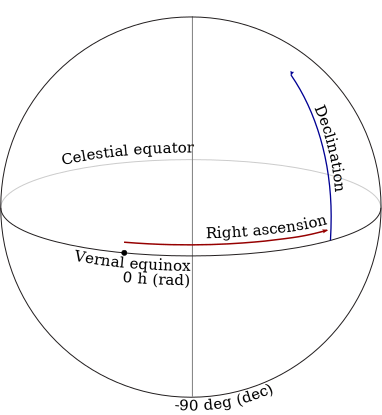
\includegraphics[width=0.5\textwidth]{images/ra-dec}
                \caption{The equatorial coordinate system used in astronomy.}
                \label{fig:equatorial-coordinates}
            \end{figure}

            Astronomy uses the \emph{equatorial coordinate system} to describe
            the positions of objects on the sky. Each position on the sky is
            described by two numbers: the \emph{right ascension} (RA) and the
            \emph{declination} (dec).

            The right ascension of an object is the angle eastward from the
            vernal equinox to the object along the celestial equator. It is
            measured in hours (h), minutes (min), and seconds (s). There are 60
            seconds in 1 minute, 60 minutes in 1 hour, and 1 hour is equal to 15
            degrees. Right ascension ranges between 0h and 24h, where both 0h
            and 24h are located at the vernal equinox. The declination of an
            object is the angle northward from the celestial equator to the
            object. It is measured in degrees (${}^\circ$), arcminutes ($'$),
            and arcseconds ($"$). Declination ranges between $-90^\circ$ and
            $90^\circ$, where $-90^\circ$ is the declination of the south
            celestial pole and $90^\circ$ is the declination of the north
            celestial pole. The right ascension and declination are shown in
            Figure \ref{fig:equatorial-coordinates}. It is important to note
            that while right ascension and declination are both measured in
            minutes and seconds, these are \emph{different} minutes and seconds.
            1 minute (right ascension) is equal to 15 arcminutes (declination).

            Objects are usually given a International Astronomical Union (IAU)
            name based on their coordinates. This name includes the catalogue
            that identified the object, the right ascension, and the
            declination. For example, ATLAS3 J002925.7-440256C is from the third
            release of the ATLAS catalogue, and is located at 00h 29m 25.7s
            $-44^\circ$ $02'$ $56"$.

        \subsection{Wavelength and Frequency}
        \label{sec:wavelength}

            Light is an electromagnetic wave, and like all waves it has
            \emph{wavelength} and \emph{frequency}. The wavelength of light is
            the distance between two neighbouring peaks; it is measured in
            metres (m) and usually denoted $\lambda$. The frequency of light is
            the number of waves per second; it is measured in hertz (Hz) and
            usually denoted $\nu$. Wavelength and frequency are related by the
            formula
            \[
                c = \lambda \nu,
            \]
            where $c$ is the speed of light.

            Humans can see a limited range of wavelengths of light. In this
            range, the wavelength of light corresponds to its colour: Blue light
            has shorter wavelength (and higher frequency) than red light.
            Outside of this range, light still has various different
            ``colours'', but we cannot see them. Different ranges of wavelength
            are assigned different names, such as infrared, x-ray, and radio.

            When objects emit light, the wavelength depends on the process by
            which the light was emitted. For example, thermal radiation is
            emitted by all objects based entirely on the temperature of the
            object, with hotter objects emitting light with shorter wavelengths.
            Another example is synchrotron radiation (Section \ref{sec:agns}),
            which is emitted in radio wavelengths.

            Since telescopes generally only detect brightnesses of objects in
            the sky, and different wavelengths of radiation require different
            mechanisms to detect, telescopes are designed to measure radiation
            only at specific ranges of wavelengths. Separate measurements of
            wavelength are later combined for analysis.

        \subsection{Flux and Magnitude}

            The \emph{flux density} of an object is its energy output per unit
            time per unit area. It is denoted $f$ and is measured in $\text{W
            m}^{-2}$. The flux density is given by
            \[
                f = \frac{1}{A}\frac{\text{d}E}{\text{d}t}
            \]
            where $E$ is the energy received from the object and $t$ is the
            time. We cannot usually measure the flux over all frequencies, so
            usually flux is observed over a specific frequency range $\Delta
            \nu$. The \emph{spectral flux density} is then the limit of this as
            the frequency range approaches zero, i.e.
            \[
                f_\nu = \frac{1}{A}\frac{\text{d}^2E}{\text{d}\nu\text{d}t}
            \]
            where $A$ is the area of the object on the sky. The spectral flux
            density is measured in janskys (Jy), an astronomical unit equal to
            $10^{-26} \text{ W m}^{-2} \text{ Hz}^{-1}$ \citep{francis08}.

            The \emph{apparent magitude}, $m$, of an object is a logarithmic
            measure of its apparent brightness seen from Earth, relative to the
            star Vega \citep{francis08}. The difference between the magnitudes
            of two objects, $m_1$ and $m_2$, represents the logarithm of the
            ratio of their flux densities
            \begin{equation}
                \label{eq:magnitude-difference}
                m_2 - m_1 = -2.5 \log_{10} \left(\frac{f_2}{f_1}\right)
            \end{equation}
            and so the apparent magnitude is given by
            \begin{equation}
                \label{eq:apparent-magnitude}
                m = -2.5 \log_{10} \left(\frac{f}{f_{\text{Vega}}}\right)
            \end{equation}
            where $f$ is the flux density of the object and $f_{\text{Vega}}$ is
            the flux density of Vega, measured at the same frequency.

    \section{Radio Active Galactic Nuclei}
    \label{sec:agns}

        \begin{figure}[!ht]
            \centering
            \includegraphics[height=0.2\textheight]
                {images/accretion_disk_artist_impression.jpg}
            \caption{An artist's impression of the accretion disk of an active
                galactic nucleus. \emph{Image: NASA/JPL-Caltech}}
            \label{fig:accretion-disk}
        \end{figure}

        Many galaxies contain a supermassive black hole in their centre
        \citep{richstone98}. These black holes may accrete matter from the
        surrounding galaxy in an \emph{accretion disk} (Figure
        \ref{fig:accretion-disk}). The accretion process emits huge amounts of
        light through different physical processes. These light-emitting black
        holes are called active galactic nuclei (AGNs). AGNs can be extremely
        bright, emitting up to $10^{39}$ J of energy every second --- nearly a
        thousand times more energy than our entire galaxy emits
        \citep{begelman84}. AGNs are found throughout the universe: The closest
        known AGN is Centaurus A (Figure \ref{fig:centaurus-a}), with a distance
        of around $2.4 \times 10^{20}$ km, and AGNs have been detected up to
        redshifts of $z \approx 7$ \citeme \todo{Convert this into a
        non-redshift distance}.

        \begin{figure}
            \centering
            \includegraphics[height=0.3\textheight]{images/M87_jet.jpg}
            \caption{M87, a giant elliptical galaxy with a jet. \emph{Image:
                NASA and The Hubble Heritage Team (STScI/AURA)}}
            \label{fig:m87}
        \end{figure}

        Around 10\% of AGNs produce \emph{jets} from their accretion disk
        \citep{fabian99}. Jets are long, thin streams of matter such as the one
        shown in Figure \ref{fig:m87}. These jets can be very large, with
        ``giant'' AGNs emitting jets nearly $1$ Mpc ($3 \times 10^{19}$ km) in
        length \citep{saripalli05}.

        Electrons in jets produce \emph{synchrotron radiation}. This is a
        form of radiation emitted by charged particles travelling at
        relativistic speeds as they accelerate in a magnetic field
        \citep{sokolov67}. Synchrotron radiation is emitted in radio
        wavelengths, and so AGNs emitting synchrotron radiation are called
        \emph{radio AGNs}. As radio AGNs are the focus of this thesis, ``AGN''
        will refer only to radio AGNs unless otherwise specified.

        \begin{figure}
            \centering
            \begin{subfigure}{0.4\textwidth}
                \includegraphics[width=\textwidth]
                    {images/FIRST_093244.58+161050.7.PNG}
                \caption{FIRSTJ093244.5+161050.}
                \label{fig:first-triple}
            \end{subfigure}%
            ~
            \begin{subfigure}{0.4\textwidth}
                \includegraphics[width=\textwidth]
                    {images/FIRST_130117.5+104121.PNG}
                \caption{FIRSTJ130117.5+104121.}
                \label{fig:first-double}
            \end{subfigure}%
            \caption{Two radio AGNs imaged by the NRAO Very Large Array.}
            \label{fig:first-agn}
        \end{figure}

        We can observe the jets of radio AGNs with radio telescopes, such as in
        Figure \ref{fig:first-agn}. The jets may appear to be separate objects,
        and there may or may not be a radio source in the middle of the AGN
        system. If the system is composed of two separate objects such as in
        Figure \ref{fig:first-double} (one object for each lobe of the jets),
        then it is called a \emph{radio double}; if a central source is also
        visible, then it is called a \emph{radio triple}.

        Since these jets are not point-like sources
        of light, and viewing the jets is the only way to observe radio AGNs,
        common astronomical problems such as cross-identification (Section
        \ref{sec:radio-cross-identification}) can be very difficult, as the true
        location of the AGN is unclear.
        % Most of the radio objects that we have seen in radio surveys conducted
        % so far are these jets \citep{norris11}. Since these jets are the only
        % way to observe radio AGNs, radio AGNs do not appear at all in surveys
        % at other wavelengths.

        % An important part of astronomical surveys is matching objects 

        % To fully understand these objects astronomers need data from more than
        % just radio surveys. Combining observations of objects in multiple
        % wavelengths is therefore a common problem in astronomy, and is called
        % \emph{cross-identification} \citep{fan15}. For point sources of light
        % this can be straightforward --- the coordinates of each source on the
        % sky are well-known and can often be immediately matched throughout
        % surveys --- but as it is the jets of AGNs that emit radio, AGNs are not
        % point sources. We discuss this in detail in Section
        % \ref{sec:radio-cross-identification}.

    \section{Radio Surveys}
    \label{sec:radio-surveys}

        A \emph{survey} is an image of the sky made with repeated observations
        in specific wavelengths, aiming to comprehensively cover some large area
        of the sky. In this section we look at EMU and ATLAS, two surveys in
        radio wavelengths that are relevant to this thesis.

        \begin{figure}
            \centering
            \includegraphics[width=0.8\textwidth]{images/skymap2.pdf}
            \caption{A map of the sky, showing the FIRST and EMU radio surveys,
                and the SWIRE infrared survey. The ATLAS radio survey
                covers both the CDFS and ELAIS-S1 fields. The WISE infrared
                survey covers the entire sky.}
        \end{figure}

        \subsection{EMU: Evolutionary Map of the Universe}
        \label{sec:emu}

            The largest existing radio survey is currently the NRAO VLA Sky
            Survey (NVSS) \citep{condon98}, which covers the entire northern sky
            as far south as $-40^\circ$. However, NVSS has low sensitivity, only
            detecting objects brighter than $2.5$ mJy. NVSS also has relatively
            low resolution, only resolving objects to $45''$. The most sensitive
            existing radio survey is of the Lockman hole \citep{owen08}, which
            only covered around $0.1$ square degrees of the sky, but detected
            objects as dim as $0.015$ mJy with an angular resolution of $1.6''$.
            The Evolutionary Map of the Universe (EMU) is an upcoming deep radio
            survey that aims to provide both high sensitivity and wide coverage
            of the radio sky \citep{norris11}. EMU will be sensitive to objects
            to around $0.015$ mJy with an angular resolution of around $10''$,
            and cover the entire southern sky as far north as $30^\circ$. The
            survey is expected to find huge numbers of radio objects --- while
            the Australia Telescope Large Area Survey [ATLAS] (which has similar
            resolution and sensitivity to EMU) has detected around 4000 radio
            objects, EMU is expected to find \emph{70 million}
            \citep{banfield15}. Such a large number of detected objects will
            make analysis of the data considerably more difficult than analysis
            of existing surveys has been. Analysis of EMU will be impossible by
            hand, and will therefore require algorithms to process the data.
            With so many new objects it is likely that many objects will not fit
            existing models, meaning that model-based approaches to data
            processing may be ineffective. It is this problem that motivates the
            development of new, machine-learned algorithms for processing
            astronomical data at these large scales. While the EMU survey data
            is not yet released, development of such algorithms can begin by
            looking at other datasets with similar sensitivity and resolution,
            such as ATLAS (Section \ref{sec:atlas}).

            EMU aims to fulfil a number of scientific goals, including:
            \begin{itemize}
                \setlength\itemsep{0 pt}
                \item investigating the evolution of galaxies and supermassive
                    black holes,
                \item exploring the large-scale structure and cosmology of the
                    universe,
                \item developing a catalogue of radio objects in the southern
                    sky,
                \item looking for never-before-seen astronomical objects, and
                \item testing strategies for dealing with data from the upcoming
                    Square Kilometre Array (SKA) telescope.
            \end{itemize}

        \subsection{ATLAS: The Australia Telescope Large Area Survey}
        \label{sec:atlas}

            \begin{figure}
                \centering
                \includegraphics[width=0.8\linewidth,]{images/CDFS_bitmap}
                \caption{ATLAS observations of CDFS.
                    Reproduced from \citet{franzen15}.}.
                \label{fig:cdfs}
            \end{figure}

            The Australia Telescope Large Area Survey (ATLAS) is a high
            sensitivity radio survey which aims to help understand the evolution
            of early galaxies \citep{norris06}. The Australia Telescope Compact
            Array was used to image two small areas of the sky: the Chandra Deep
            Field South (CDFS), and the European Large Area ISO Survey - South 1
            (ELAIS-S1) field. CDFS and ELAIS-S1 are areas of the sky with few
            nearby objects, meaning that observations in these fields are of
            very old, distant objects. These fields in particular were chosen
            because they are the two fields imaged in the Spitzer Wide-area
            Infrared Extragalactic Survey (SWIRE, Section \ref{sec:swire})
            visible from the southern hemisphere. SWIRE produced high-resolution
            infrared images of its fields, allowing all objects detected in the
            ATLAS radio images to be cross-identified with their infrared
            counterparts.

            ATLAS is considered a pilot survey for EMU. EMU and ATLAS image the
            same wavelengths with similar resolution and sensitivity, so tools
            and methods developed to process and interpret ATLAS data are
            expected to work well on the data produced by EMU.

            ATLAS provides both a catalogue of detected radio objects and a
            radio image of the CDFS and ELAIS-S1 fields. The CDFS image covers a
            total area of 3.7 square degrees and the ELAIS-S1 image covers a
            total area of 2.7 square degrees. The CDFS image is shown in Figure
            \ref{fig:cdfs}. The catalogue is a list of all objects detected in
            the images with a peak or integrated flux more than 5 times the
            background noise levels. For each object, the catalogue lists
            \begin{itemize}
                \setlength\itemsep{0 pt}
                \item an survey identifier,
                \item an IAU name,
                \item a position on the sky of the peak flux,
                \item a peak flux density,
                \item an integrated flux density,
                \item an angular size,
                \item whether the object is extended or compact, and
                \item a spectral index,
            \end{itemize}
            as well as uncertainties associated with each measurement
            \citep{franzen15}.

            The ATLAS survey of the CDFS field is the focus of experiments in
            this thesis, for three main reasons. It contains around 2400
            objects, providing enough training data for machine learning
            methods, but still remaining a manageable size for our
            resource-limited tests. As a pilot survey for EMU, we expect methods
            developed on ATLAS to also work on EMU. Finally, we have three sets
            of cross-identifications for ATLAS-CDFS (see Sections
            \ref{sec:radio-cross-identification} and
            \ref{sec:radio-galaxy-zoo}), allowing us to check the performance of
            methods we develop.

    \section{Infrared Surveys}
    \label{sec:infrared-surveys}

        \subsection{WISE: Wide-field Infrared Survey Explorer}
        \label{sec:wise}

            \begin{figure}
                \centering
                \includegraphics[width=0.5\textwidth]
                    {images/WISE_3h30m05.24s-28d34m46.3s.png}
                \caption{Patch of the WISE multi-wavelength composite image
                    centred on 3h30m05.24s -28d34m46.3s.}
                \label{fig:wise}
            \end{figure}

            The Wide-field Infrared Survey Explorer (WISE) is an orbital
            infrared telescope. In 2009--2010 it was used to survey the entire
            sky in four wavelengths: 3.4 $\mu$m, 4.6 $\mu$m, 12 $\mu$m, and 22
            $\mu$m. These wavelengths are referred to as WISE bands $w1$, $w2$,
            $w3$, and $w4$, respectively. WISE images have resolutions of
            $6''$--$12''$, with sensitivity between $0.08$ and $6$ mJy,
            corresponding to the detection of sources between $16.5$ and $7.9$
            magnitude \citep{wright10}.

            The AllWISE catalogue \citep{cutri13} is the most recent WISE
            catalogue. For each object detected, the catalogue includes the
            magnitudes in each WISE band, as well as a number of other features
            we do not make use of in this thesis. We will refer to the
            magnitudes in each band by the names of the bands (i.e. $w1$ --
            $w4$).

            The main goal of WISE was to provide a map of the whole sky in
            infrared wavelengths for many different reasons: infrared
            measurements may be used to detect and classify distant galaxies,
            measurements can be cross-identified to complement other surveys,
            and so on. There are many other scientific goals of WISE; these are
            described in detail by \citet{wright10}.

        \subsection{SWIRE: Spitzer Wide-area Infrared Extragalactic Survey}
        \label{sec:swire}

            \begin{figure}
                \centering
                \includegraphics[width=0.5\textwidth]{images/swire_small.jpg}
                \caption{Patch of the SWIRE multi-wavelength composite image
                    centred on 3h30m05.24s -28d34m46.3s. This is the same region
                    of the sky as the WISE image in Figure \ref{fig:wise}.}
            \end{figure}

            The Spitzer Wide-Area Infrared Extragalactic Survey (SWIRE) is an
            infrared survey of seven fields of the sky
            \citep{lonsdale03}. These fields --- ELAIS-S1, ELAIS-N1, ELAIS-N2,
            Lockman, CDFS, and Lonsdale --- are called the \emph{SWIRE fields},
            totalling 63.2 square degrees in area. ELAIS-S1 and CDFS are in the
            southern sky; all other fields are in the northern sky. SWIRE is a
            multi-wavelength survey, observing at four wavelengths: 3.6 $\mu$m,
            4.5 $\mu$m, 5.8 $\mu$m, and 8.0 $\mu$m.

            While SWIRE covers far less area of the sky than WISE, it does so at
            considerably higher resolution and sensitivity: $1.2''$ and
            $7.3$--$32.5$ $\mu$Jy, respectively
            \citep{irac-pocket-guide, surace05}.

            SWIRE aimed to investigate the evolution of galaxies and AGNs and
            the relationship between galaxies and AGNs \citep{surace05}.

    \section{Radio Cross-identification}
    \label{sec:radio-cross-identification}

        % \subsection{Motivation}
        % \label{sec:cross-identification-motivation}

        Observations of astronomical objects in different wavelengths give us
        information on different physical properties of the objects. We can only
        make use of this information, however, if we can match observations of
        the same object in different surveys. This is called
        \emph{cross-identification}.

        The specific cross-identification task we focus on in this thesis is
        that of cross-identifying a radio object with its infrared counterpart.
        Most often in current radio surveys, a radio object will be a jet from
        an AGN \citep{norris11}. In this case, we refer to the infrared
        counterpart as the \emph{host galaxy} of the AGN. In this thesis we will
        assume that all radio objects are AGNs.
        The main goal of cross-identifying AGNs is to better understand the
        relationship between AGNs and star-forming activity in their host
        galaxies \citep{norris06}.

        Sometimes, cross-identification is easy: We may have point-like sources
        of light, and we can simply overlay two surveys and identify overlapping
        objects. In the case of cross-identifying radio AGNs, though, we do not
        have point-like sources of light, and cross-identification can be very
        difficult. AGN jets may be arbitrarily large and complex, and often show
        up as multiple disconnected radio objects. As such, past attempts to
        cross-identify radio objects have required human insight
        \citep{norris06,fan15}.

        In this section, we look at two different ways astronomers have
        cross-identified radio objects in the CDFS field of the ATLAS survey. We
        will make use of the resulting catalogues later in this thesis.

        % While we cannot observe the black holes of AGNs directly, we can observe
        % the radio emissions from their jets. These could then be matched to the
        % galaxies hosting the black holes, allowing us to learn more about the
        % galaxy, the black hole, and the surrounding environment. These host
        % galaxies are not visible in radio wavelengths,

        \subsection{Norris et al. Catalogue}
        \label{sec:norris}

            Along with a catalogue of radio objects found in the CDFS field by
            the ATLAS survey, \citet{norris06} produced a catalogue of
            cross-identifications of these radio objects. The catalogue lists
            ATLAS objects and their corresponding SWIRE objects.

            The cross-identification process was semi-automated.
            \citeauthor{norris06} first matched each ATLAS object to the nearest
            SWIRE object. After this step, around half of the radio objects were
            matched to a SWIRE object within $1''$, and $79\%$ were matched to a
            SWIRE object within $3''$. Radio objects greater than $3''$ away
            from a SWIRE object were then cross-identified manually; radio
            doubles and radio triples were matched to the SWIRE object nearest
            their centre.

            Additionally, \citeauthor{norris06} found between 8 and 22 radio
            objects with no identifiable host galaxy in the infrared. These are
            called ``infrared-faint'' radio objects.

            \citeauthor{norris06} estimated the probability of false cross-
            identifications by displacing all radio objects by $1'$ and
            repeating the cross-identification process. From the results of this
            test, they estimated that $9.02\%$ of the cross-identifications are
            false.

            We consider these cross-identifications \emph{expert} cross-
            identifications, i.e., they are the best possible cross-
            identifications available for radio objects in the CDFS field.
            Throughout this thesis, we will use these as an approximation to the
            unobservable groundtruth cross-identifications.

        \subsection{Fan et al. Catalogue}
        \label{sec:fan}

            \citet{fan15} developed an automated cross-identification algorithm
            that fits astronomical models of AGNs to the radio sky.

            The algorithm examines each infrared object in turn. Under the
            assumption that the infrared object is a host galaxy, it then
            searches in a $2'$ radius for potential radio components of AGN
            jets. The radio components with highest likelihood according to a
            Bayesian model are selected using a greedy algorithm.

            This method has some clear limitations --- it is model-based, and
            thus may fail for unexpected radio objects like those we might find
            in EMU, and it is not able to cross-identify infrared-faint radio
            objects. Nevertheless, it performs very well when applied to the
            ATLAS-CDFS field, making 564 cross-identifications identically to
            \citeauthor{norris06}, missing 31 cross-identifications that
            \citeauthor{norris06} reported, and cross-identifying an additional
            62 radio objects.

            In this thesis, we consider the \citeauthor{fan15}
            cross-identifications of ATLAS-CDFS as an alternative source of
            expert cross-identifications, due to the high (but not total)
            agreement with \citeauthor{norris06}.

    \section{Radio Galaxy Zoo}
    \label{sec:radio-galaxy-zoo}

        \begin{figure}
            \centering
            \begin{subfigure}[t]{0.3\textwidth}
                \centering
                \includegraphics[height=2in]{images/rgz_radio.png}
                % These empty captions give us something to reference later.
                \caption{}
                \label{fig:rgz-interface-a}
            \end{subfigure}%
            ~
            \begin{subfigure}[t]{0.3\textwidth}
                \centering
                \includegraphics[height=2in]{images/rgz_ir.png}
                \caption{}
                \label{fig:rgz-interface-b}
            \end{subfigure}%
            ~
            \begin{subfigure}[t]{0.3\textwidth}
                \centering
                \includegraphics[height=2in]{images/rgz_done.png}
                \caption{}
                \label{fig:rgz-interface-c}
            \end{subfigure}
            \caption{Radio Galaxy Zoo volunteer workflow.\\
                \protect\makebox[1.5cm][r]{\ref{fig:rgz-interface-a}}
                    Volunteers are first asked to identify associated radio
                    objects.\\
                \protect\makebox[1.5cm][r]{\ref{fig:rgz-interface-b}}
                    Volunteers then cross-identify the radio objects with the
                    corresponding host galaxy.\\
                \protect\makebox[1.5cm][r]{\ref{fig:rgz-interface-c}}
                    This is repeated for all radio objects in the image.}
            \label{fig:rgz-interface}
        \end{figure}

    The \citeauthor{norris06} catalogue is highly accurate, but manual expert
    cross-identification of radio surveys is impractical for large surveys. The
    CDFS field examined by \citeauthor{norris06} only contains around 2400 radio
    objects, which is small even compared to existing surveys (e.g. Faint Images
    of the Radio Sky at Twenty-Centimeters (FIRST) \citep{becker95} found
    946~000 radio sources). Automated algorithms such as \citeauthor{fan15}
    scale better, but most such algorithms are still in their infancy
    \citeauthor{norris16} and many are model-based, potentially missing many
    sources that do not fit the models. The Radio Galaxy Zoo project
    \citep{banfield15} provides a different approach: Allow many non-expert
    volunteers to manually cross-identify radio sources with their infrared host
    galaxies.

    Radio Galaxy Zoo is a website where volunteers are presented with a radio
    image from ATLAS or FIRST and a corresponding infrared image from SWIRE or
    WISE, and are tasked with matching the radio source with its host galaxy, as
    well as identifying which radio objects are associated with the same host
    galaxy (e.g., two radio objects may represent two jets of one AGN). To help
    reduce noise in these matches, each compact radio object is shown to 5
    volunteers, and each complex radio object is shown to 20 volunteers. While
    both the cross-identification task and the radio object association task are
    astronomically interesting, we focus only on the cross-identification task
    for this thesis. An example of the workflow presented to volunteers is shown
    in Figure \ref{fig:rgz-interface}.

    Since its launch in December 2013, the Radio Galaxy Zoo project has labelled
    over 100~000 radio objects. One particularly notable result is the discovery
    of one of the largest known wide-angled tail AGNs by two volunteers, which
    would be impossible to detect in current automated algorithms
    \citep{banfield16}.

    The Radio Galaxy Zoo dataset contains around 177~000 images from FIRST, and
    2400 images of the CDFS field from ATLAS. The ATLAS images of the ELAIS-S1
    field are not included, and may be used as a testing set for
    cross-identification algorithms trained on the Radio Galaxy Zoo in the
    future. Each image is a 2 arcminute-wide square.

    The cross-identifications are stored in a MongoDB database as a collection
    of associated radio objects and the corresponding pixel locations of the
    volunteers' clicks, as well as the right ascension and declination of the
    radio object. The radio and infrared image patches associated with each
    radio object are also included alongside the database. For detailed analysis
    of these labels, see \citet{atlas-ml}.

    In this thesis, we will train machine learning algorithms to perform the
    cross-identification task trained on ATLAS-CDFS labels from the Radio Galaxy
    Zoo.

%     Radio Galaxy Zoo volunteers are first asked to select combinations of
%     radio objects that correspond to one radio source, and are then asked to
%     select the location of the corresponding host galaxy \citep{banfield15}.
%     Each radio subject is labelled by multiple volunteers. These labels are
%     then collated as follows. First, the most common combination of radio
%     objects is selected, and all labels that have a different combination are
%     discarded. This radio combination is called the consensus radio
%     combination. Then, the density of host location labels is estimated using
%     Gaussian kernel density estimation (KDE), and the highest density location
%     is selected. This is called the consensus host location. The consensus
%     host location is then matched to the nearest infrared object.

%     An alternative way to find the consensus host location is by using a
%     clustering algorithm such as $k$-means. Host locations are clustered and
%     the cluster containing the most locations is taken to represent the
%     consensus; the consensus location is then the mean of the cluster. This is
%     faster and more robust than using KDE, but requires $k$ to be known. $k$
%     can be estimated using an algorithm such as PG-means \citep{hamerly07} or
%     by choosing $k$ to minimise some information criterion
%     \todo{cite:sklearn}. The consensus labels for the data associated with
%     this thesis were found in this way, fitting a Gaussian mixture model to
%     the host locations with the number of Gaussians chosen to minimise the
%     Bayesian information criterion.

%     Repeated volunteer labelling helps to reduce noise in the labels. This is
%     necessary as the volunteers are not experts, and may incorrectly label the
%     subject. The hope is that the majority of volunteers will correctly label
%     subjects, which seems to be the case for radio subjects where more than
%     75\% of volunteers agree \citep{banfield15}. The number of times a radio
%     subject is shown to different volunteers is called the redundancy. The
%     redundancy is 5 if the subject is a compact source, and 20 for all other
%     sources. These numbers were chosen based on the redundancy levels of the
%     original Galaxy Zoo project [Banfield, personal communication] \todo{Is
%     this how to cite personal communication? Alternatively, is this written
%     down somewhere?}. Since labels with radio combinations that disagree with
%     the consensus are discarded, the redundancy is usually lower in practice
%     when finding the host location. This can lead to very low redundancy input
%     to KDE, causing KDE to fail. This failure can usually be caught, but the
%     existing solution in this case is to take the mean of all host locations.
%     This is not the consensus host location in general. Another effect is that
%     since more complex sources have higher levels of disagreement in the radio
%     combination stage, more complex sources have more discarded volunteer
%     labels, and thus lower redundancy --- so more complex sources have more
%     noise in their labels.

\chapter{Machine Learning}

\begin{enumerate}
    \item something about machine learning, classification, regression
    \item something about active learning, pool-based active learning
\end{enumerate}

%!TEX root=thesis.tex

\chapter{Radio Cross-identification}
\label{cha:passive-learning}
  % In this chapter I'll talk about a machine learning approach to the cross-identification problem (i.e. my pipeline).

  In this chapter, I develop a machine learning approach to the radio cross-identification problem. First, I will discuss different ways to train and use a classifier for the task, in particular framing the cross-identification problem as an object localisation problem. Then, I will discuss the available training data and how I chose to process it. Finally, I will present results against a dataset of expert labels, and compare these results to those found by other methods.

\section{Formalism}
\label{sec:cross-identification-formalism}
  
  \todo{Rewrite below into this section.}

  \todo{Explain why we're ignoring the radio part of this problem.}

  \subsection{Cross-identification as Object Localisation}
  \label{sec:object-localisation}

  \subsection{The Galaxy Classification Task}
  \label{sec:galaxy-classification-task}

% \section{Cross-identification as Binary Classification}
% \label{sec:framing-as-classification}
  
  When we look at the sky with radio telescopes, we see the radio emissions from
  the jets of AGNs. \todo{Add backlink.} Given an image of these radio
  emissions, we want to locate the host galaxy containing the associated AGN. In
  general, there may be multiple hosts associated with one radio object (such as
  in Figure \ref{fig:two-hosts}), but we make the assumption that there is only
  one. This is the same assumption made by Radio Galaxy Zoo \todo{cite:rgz-
  analysis-github(?)} and greatly simplifies the problem.

  \begin{figure}[!ht]
    \centering
    \includegraphics[width=0.5\textwidth]{images/CI0370C1_heatmap+contours.png}
    \caption{A radio object (ARG0003ra1) with two host galaxies. This radio
      object is actually two radio objects that have been incorrectly detected
      as one, and there is one host galaxy for each object.}
    \label{fig:two-hosts}
  \end{figure}

  We can interpret cross-identification as an object localisation problem. As
  input, we have an image of the radio sky, and we want to locate a host galaxy
  in this image. A common way to find an object in an image is by using a
  sliding window. A fixed-size image patch centred on each pixel is taken as a
  feature representation of that pixel. This is then used as input to a
  classification model which outputs a probability for each pixel, with higher
  probabilities corresponding to higher likelihood of the object being located
  at that pixel. The pixel with the highest rating is considered the location
  of the object. This approach can be improved by intelligently selecting
  candidate pixels and only testing these. For the cross-identification
  problem, we can use galaxy locations as candidate pixels, with galaxies found
  in infrared surveys such as WISE and SWIRE. Additionally, astronomical
  measurements such as flux are included in these surveys and these may be
  taken as additional features for each candidate pixel, giving more
  information to the classifier.

  This approach can be formalised as follows. Consider a set $\mathcal X$ of
  candidate host galaxies, and a radio object $r$ that we want to assign a
  host galaxy. Let $y : \mathcal X \to \{0, 1\}$ represent whether a given $x
  \in \mathcal X$ is the host galaxy associated with $r$. Under the assumption
  that a radio object has exactly one associated host galaxy, then there exists
  exactly one $x \in \mathcal X$ such that $y(x) = 1$, and for all other $x \in
  \mathcal X$, $y(x) = 0$. The cross-identification task then amounts to
  modelling $p(y(x) = 1 \mid x, r)$. Once this distribution is modelled, the
  host galaxy associated with $r$ is given by
  \begin{equation}
      \label{eq:cross-identification}
      \mbox{host}(r) = \underset{x}{\mbox{argmax}}\ p(y(x) = 1 \mid x, r).
  \end{equation}

  Ideally, $\mathcal X$ is the set of all galaxies. This is clearly
  intractable, so as an approximation we use a catalogue of infrared objects
  near the radio object of interest, taken from an infrared survey. We also
  make the assumption that the host galaxy is within $1'$ of the radio object
  --- while this doesn't hold in general, systems larger than $1'$ are rare and
  require human insight to discover \citep{banfield16}.

\section{Evaluating Performance Without Groundtruth}
\label{sec:norris-as-groundtruth}
  
  \todo{Write about Norris intersection Fan labels.}

\section{Feature Selection}
\label{sec:features}

  To train a machine learning method to solve the galaxy classification task,
  we must find a representation of galaxies in a feature space $\mathbb{R}^D$.
  In this section we describe and motivate our choice of galaxy features,
  extracted from both infrared and radio surveys.

  \subsection{Infrared Features}
  \label{sec:ir-features}

    The WISE catalogue (Section \ref{sec:wise}) contains magnitude information
    for each object. There are four such magnitudes --- $w1$, $w2$, $w3$, and
    $w4$ --- each representing the amount of light emitted by the object in a
    different range of wavelengths.

    We chose to use all four magnitudes as features. Since the features are
    magnitudes, they are on a logarithmic scale, and we found that in practice
    classification performance improved when the magnitudes were converted to
    fluxes. We performed this conversion with the formula
    \[
      f = 10^{-0.4m}
    \]
    where $f$ is the flux and $m$ is the magnitude. This is the inverse of
    Equation \ref{eq:apparent-magnitude}, and gives the flux in arbitrary, but
    linear, units.

    \begin{figure}[!ht]
      \centering
      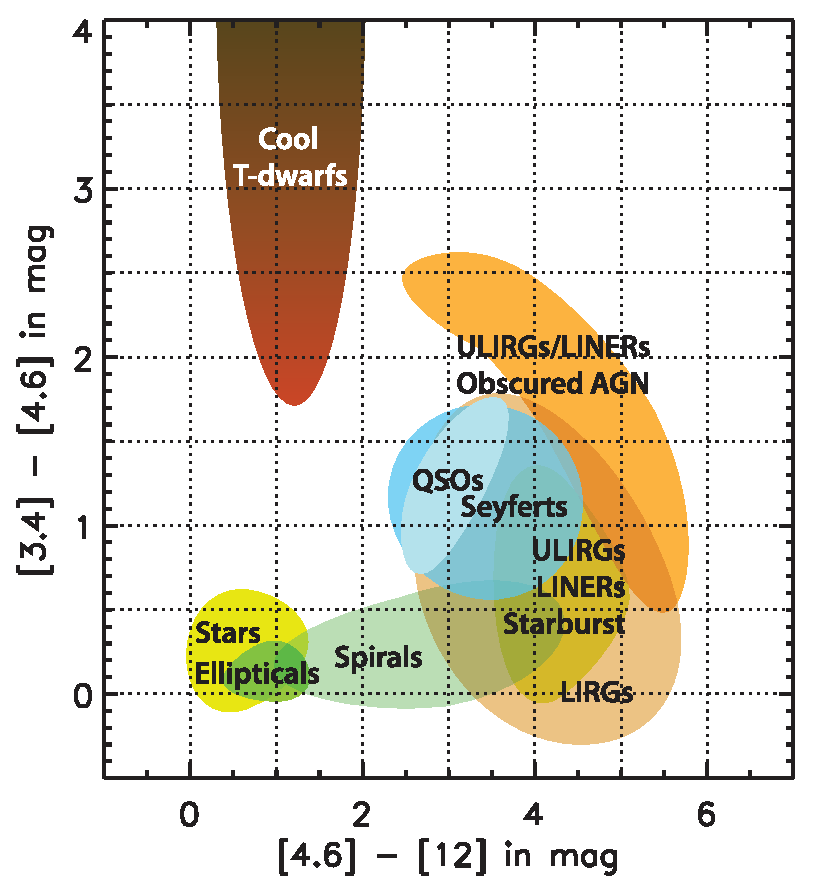
\includegraphics[width=0.5\textwidth]{images/wise_colour-colour}
      \caption{WISE colour-colour diagram showing the colours of various
        astronomical objects. The horizontal axis is $w2 - w3$ and the vertical
        axis is $w1 - w2$. Reproduced from \citep{wright10}.}
      \label{fig:wise-colour-colour}
    \end{figure}

    The ratios between infrared fluxes are indicators of physical galactic
    properties such as star formation and dust \todo{Find a source on this ---
    Probably the WISE paper wright10}. In practice, the $w1 - w2$ and $w2 - w3$
    ratios are most commonly used (such as in Figure
    \ref{fig:wise-colour-colour}), so we chose to use these ratios as features.
    Once again, we used a linear scale, computing the ratios using equation
    \ref{eq:magnitude-difference}.

    Also available were the unprocessed infrared images captured in the survey.
    Under the assumption that the large scale infrared structure of a galaxy is
    unchanged by an AGN, we chose to ignore the images themselves and focus on
    features obtained from the catalogue. This greatly simplified feature
    selection with minimal expected impact on the classification performance.
    Future work may investigate the effectiveness of features extracted from
    infrared images on classification performance, but this is out of the scope
    of this thesis.

    \todo{Discuss SWIRE features.}

    % The SWIRE catalogue (Section \ref{sec:swire}) also contains colour
    % information for each contained object, but only fluxes rather than
    % magnitudes. \todo{Read the SWIRE colour-colour diagram and continue this.}

    % Both WISE and SWIRE catalogues contain the positions of each object. The
    % distance from each object to the centre of the closest radio object is
    % used as a feature representing that object. This noticeably improves
    % classification performance \todo{make an experiment showing this, and
    % probably also showing that the other features are good}.

  \subsection{Radio Features}
  \label{sec:image-features}

    While the infrared catalogues include measurements on individual galaxies,
    the ATLAS radio catalogue does not. This is because galaxies are not
    visible in radio, so while galaxies are directly represented in an infrared
    catalogue they are not in a radio catalogue. Galactic features must thus be
    extracted from the radio images directly. We chose to use a convolutional
    neural network, as described in Section \ref{sec:image-features}.

    \subsubsection{Building a Model for Feature Extraction}
    \label{sec:feature-extraction-model}

      We chose to use a convolutional neural network (CNN) with three
      convolutional and max pooling layers, shown in Figure \ref{fig:radio-cnn}.
      This resulted in an 128-dimensional feature vector. For training this
      network, we added a 64-dimensional dense layer mapping to a 1-dimensional
      output. 10\% of ATLAS objects were selected at random and reserved for
      training the CNN, to ensure later testing data would not overlap the
      training set. The entire network was then trained to match the consensus
      Radio Galaxy Zoo labels of the galaxies nearest the reserved training set.

      \begin{figure}[!ht]
         \centering
         \includegraphics[width=\textwidth]{images/cnn_new.pdf}
         \caption{Convolutional neural network for radio feature extraction.}
         \label{fig:radio-cnn}
       \end{figure}

      A better approach would be to use a convolutional autoencoder, which would
      allow training on all the radio data, and data with no labels at all, but
      this was computationally infeasible for this project.

      An example of the neural network applied to a radio image is shown in
      Figure \ref{fig:rgz-cnn}.

      \begin{figure}[!ht]
        \centering
        \includegraphics[width=\textwidth]{images/rgz_cnn}
        \caption{The effects of convolutional layers on an input image. The
          left-most image is the original radio image. The other images are the
          32 images output from each of the three convolutional layers.}
        \label{fig:rgz-cnn}
      \end{figure}

  \subsection{Feature Analysis}
  \label{sec:feature-analysis}

    To determine the effect of each set of features on classification
    performance, we performed a feature ablation experiment. We trained a
    logistic regression classifier on the \citeauthor{norris06} label set,
    holding out different features each time. The lower the resulting balanced
    accuracy, the more important the held out features. This was repeated ten
    times with different $50\%$ subsets of the training set. The features we
    chose to hold out were all features derived from magnitudes, all features
    extracted by the CNN, the distance feature, and each magnitude feature
    individually. These results are plotted in Figure \ref{fig:feature-ablation}
    and the means and standard deviations of the balanced accuracies are tabled
    in Table \ref{tab:feature-ablation}.

    \begin{figure}[!ht]
      \centering
      \includegraphics[width=\textwidth]{%
        images/experiments/feature_ablation.pdf}
      \caption{Balanced accuracy of logistic regression trained on the
        \citeauthor{norris06} label set with different features removed. The
        horizontal axis indicates which features were removed for the results
        in that column.}
      \label{fig:feature-ablation}
    \end{figure}

    \begin{table}[!ht]
      \centering
      \begin{tabular}{r|c}
        \textbf{Feature/s Removed} & \textbf{Mean Balanced Accuracy}\\\hline
        All magnitudes & $(88.66 \pm 0.81)\%$\\
        CNN & $(71.67 \pm 1.71)\%$\\
        Distance & $(88.84 \pm 0.76)\%$\\
        $w1$ & $(88.82 \pm 0.78)\%$\\
        $w1 - w2$ & $(88.78 \pm 0.85)\%$\\
        $w2$ & $(88.79 \pm 0.80)\%$\\
        $w2 - w3$ & $(88.82 \pm 0.70)\%$\\
        $w3$ & $(88.79 \pm 0.77)\%$\\
        $w4$ & $(88.74 \pm 0.77)\%$
      \end{tabular}
      \caption{Balanced accuracy of logistic regression trained on the
        \citeauthor{norris06} label set with different features removed.}
      \label{tab:feature-ablation}
    \end{table}

\section{Choosing a Binary Classifier}
\label{sec:binary-classifiers}
  
  \begin{figure}[!ht]
    \centering
    \includegraphics[width=\textwidth]{images/experiments/lr_rf}
    \caption{Comparison of logistic regression and random forests on the galaxy
      classification task, trained on the \citet{norris06} and \citet{fan15}
      label sets, and tested against the \citet{norris06} label set.}
  \end{figure}

  To compare the performance of logistic regression with random forests on the
  galaxy classification task, I performed the following experiment. First, I
  generated five test sets of WISE objects. Then, using all other WISE objects
  as a training set, I trained a logistic regression classifier for each test
  set, first using labels from \citet{norris06}, and then, separately, using
  labels from \citet{fan15}. I then computed the balanced accuracy for each
  classifier. Finally, I repeated the experiment for random forests.

  To generate the test sets, I first selected at random half of all ATLAS
  objects. I then added all WISE objects within $1'$ of a selected ATLAS object
  to the test set. This was repeated for each test set. The motivation for first
  selecting ATLAS objects rather than drawing WISE objects directly is that WISE
  objects have overlapping features since radio features are taken from a patch
  of sky centred on each object, and WISE objects tend to be close together.
  Objects from the test sets were then removed at random until all test sets
  were the same size. Each test set contained $13605$ WISE objects.
  \todo{Check numbers.}

\section{Handling Crowd Labels}
\label{sec:rgz-crowd-labels}

  While we want to train a classifier on the crowdsourced labels from the Radio
  Galaxy Zoo, it is unclear how we should aggregate the labels. Some methods for
  aggregation are described in Section \ref{sec:crowd-labels}. Which method will
  perform best on a dataset is dependent on the dataset itself, so we tested
  both variants of the \citeauthor{raykar10} algorithm and majority vote on the
  galaxy classification task.

  \todo{Compare majority vote and Raykar.}

\section{Results}
\label{sec:rgz-results}
  
  \subsection{Classifying Galaxies}

    \todo{Make this writing considerably less terrible.}

    The infrared objects were partitioned into a testing set and a training set
    as follows. First, the radio objects were partitioned into a radio testing
    set and a radio training set, with the radio testing set containing $452$
    objects and the radio training set containing $1811$ objects. Infrared
    objects were then added to the infrared testing set if they were within $1'$
    of a radio object in the radio testing set, and added to the infrared
    training set otherwise. This was done because infrared objects that were
    close together had overlapping radio features, and thus random partitioning
    would result in the training set containing many of the features found in
    the testing set. The partitioning resulted in $5922$ objects in the testing
    set and $18218$ objects in the training set.

    For each infrared object, features and labels were generated as described in
    Sections \ref{sec:features} and \ref{sec:consensuses}, respectively. Note
    that the labels were sourced from the Radio Galaxy Zoo. A logistic
    regression classifier was then trained on the training set using binary
    cross-entropy loss, with loss of each data point weighted based on the
    frequency of its label.

    The classifier was then used to classify the objects in the testing set. The
    labels were compared to those found by \citet{norris06} as described in
    Section \ref{sec:norris}, resulting in $80.14\%$ balanced accuracy.
    \todo{This number is out of date.}

    \todo{ROC/precision--recall curves}

    \begin{figure}[!ht]
      \centering
      \includegraphics[width=\textwidth]{images/experiments/predictors.pdf}
      \caption{Performance of logistic regression on the galaxy classification
        task, trained on different sets of labels and tested on the galaxies
        where \citeauthor{norris06} and \citeauthor{fan15} labels agree. LR($Y$)
        indicates logistic regression trained on $Y$. RGZ-MV is the set of
        majority vote labels from the Radio Galaxy Zoo. RGZ-Raw-MV is the
        majority vote of all crowd labels and is included for comparison.}
    \end{figure}

  \subsection{Number of Training Examples}

    \begin{figure}[!ht]
      \centering
      \includegraphics[width=\textwidth]{images/experiments/passive.pdf}
      \caption{Performance of logistic regression on the galaxy classification
        task, trained on different amounts of the \citeauthor{norris06} label
        set.}
    \end{figure}

\section{Discussion}
\label{sec:rgz-discussion}
%!TeX root=./thesis.tex

\chapter{Active Learning}
\label{cha:active-learning}

In this chapter we discuss active learning and look at its application to both
the galaxy classification task and to the Radio Galaxy Zoo project.

\section{Introduction}
\label{sec:intro-active-learning}
    
    In supervised learning we deal with a set of data points and their
    associated labels. This dataset may be expensive to obtain, but the main
    costs may come from collecting labels, rather than from collecting the data
    points themselves. Examples of such data include text samples
    \citep{lewis94, mccallum98}, and images \citep{loy11, lintott08}, both of
    which are now widely and cheaply available through the internet. A more
    abstract example is scientific hypotheses \citep{king04}. Labelling text and
    images is hard, error-prone, and requires humans; and performing a
    scientific experiment to test a hypothesis is considerably more expensive
    than coming up with the hypothesis. It may even be the case that we simply
    cannot label all the data because there is too much, such as in the Galaxy
    Zoo \citep{lintott08} and Radio Galaxy Zoo \citep{banfield15} projects.

    \emph{Active learning} (or \emph{query learning} \citep{settles09, seung92,angluin86})
    allows a machine learning algorithm to select specific, unlabelled examples
    to be labelled by an expert. The algorithm effectively chooses its own
    training set \citep{settles09}. The hope is that the algorithm can choose to
    label only the most useful examples \citep{mccallum98}, and the expensive
    process of labelling redundant or useless examples is avoided
    \citep{engelson99}. Intelligently selecting the training set as in active
    learning can result in massively reduced labelling costs \citep{lewis94,
    king04} or even make intractable labelling problems tractable.

    While there are many variations of active learning scenarios, we focus on
    \emph{pool-based} active learning in this thesis. In pool-based active
    learning, we already have a large pool of unlabelled data points accessible
    to our algorithms, and our algorithms can choose to present any of these
    data points to the expert. The pool-based scenario commonly arises when we
    are able to obtain a lot of unlabelled data at once, such as in astronomical
    surveys \citep{pelleg04, richards12, marshall15}.

    Active learning has already been successfully applied in astronomy.
    \citet{pelleg04} applied active learning to the Sloan Digital Sky Survey to
    find anomalies in the survey. \citet{richards12} applied active learning to
    classify variable stars from the All Sky Automated Survey. Both papers
    showed that active learning resulted in a great reduction in the number of
    labels needed to achieve their respective tasks.

\section{Query Strategies}
\label{sec:query-strategies}

    A \emph{query strategy} is the approach an active learning algorithm takes
    to selecting a new data point to label. There are many different query
    strategies, but here we focus on uncertainty sampling and
    query-by-committee.

    All pool-based query strategies take the same form. We are given some pool
    of data $\mathcal X$ and a set of labelled data $\mathcal D = \mathcal X
    \times \mathcal Y$. We want to select $\tilde x \in \mathcal X$ such that
    labelling $\tilde x$ maximises our information gain.

    \subsection{Uncertainty Sampling}
    \label{sec:uncertainty-sampling}

        \emph{Uncertainty sampling} \citep{lewis94} is perhaps the most common
        query strategy. Given a classification model $y(\vec x) = p(z \mid x)$
        with the ability to output a probability (including probabilistic
        classifiers like logistic regression, nearest-neighbour classifiers
        \citep{lewis94}, and combinations of probabilistic and non-probabilistic
        classifiers \citep{lewis94b}), the queried point $\tilde x$ is the data
        point for which the model is least certain of the classification. This
        is not well-defined and an uncertainty sampling algorithm must choose
        what ``least certain'' means. There are three common measures of
        uncertainty --- confidence-, entropy-, and margin-based --- but in the
        case of binary classification, they all reduce to one strategy
        \citep{settles09}:
        \[
            \tilde x = \underset{\vec x}{\mbox{argmax}}\ 1 - \abs{y(\vec x) - 0.5}.
        \]
        The intuition is that the further a data point is from the decision
        boundary, the more certain the classifier is of the assigned label, so
        choosing the closest data point to the decision boundary is equivalent
        to choosing the most uncertain data point. Another interpretation is that $1 - \abs{y(\vec x) - 0.5}$ is the expected probability of mislabelling $\vec x$ \citep{settles09}.

        % In the confidence-based approach, $\tilde x$ is the data point that is
        % closest to the decision boundary, i.e.

        % % In the 

    \subsection{Query-by-Committee}
    \label{sec:qbc}

        Query-by-committee (QBC)

\section{Query-by-Committee on the Galaxy Classification Task}
\label{sec:rgz-qbc}

    We tested QBC active learning on the galaxy classification task described in Chapter \ref{cha:cross-identification}, comparing QBC to passive (i.e. random) selection as a query strategy.

    We used a committee of 20 logistic regression classifiers for the QBC test.
    Each was presented with 75\% of the known labels at random, stratified by the labels.

    For the passive test, we sampled 100 galaxies at random (stratified by the
    labels) and trained a logistic regression classifier on these. We then drew
    a batch of new labels, added these to the existing label set, and then
    retrained the classifier. This was repeated until the classifier had seen
    the entire training set ($10^4$ labels). The process for testing QBC was
    identical, except that instead of drawing new labels at random, the new
    labels were drawn in order of highest to lowest disagreement of the
    committee.

    \begin{figure}
        \centering
        \includegraphics[width=0.8\textwidth]
            {images/experiments/rgz_qbc.pdf}
        \caption{Logistic regression trained on the \citeauthor{norris06}
            labels with different amounts of training data and two different
            query strategies.}
        \label{fig:rgz-qbc}
    \end{figure}


%% Conclusion
%%
%% Template conclusion.tex
%%

\chapter{Conclusion}
\label{cha:conclusion}

\section{Why this is a Very Clever Thesis}
\label{sec:why}

%%% Local Variables: 
%%% mode: latex
%%% TeX-master: "thesis"
%%% End: 


%%%%%%%%%%%%%%%%%%%%%%%%%%%%%%%%%%%%%%%%%%%%%%%%%%%%%%%%%%%%%%%%%%%%%%
% End text.

%!TeX1 root=thesis.tex

\appendix
\chapter{Crowdastro Package}

As part of this thesis, we developed an open source Python package called
\emph{crowdastro}, containing methods for machine learning on the cross-
identification task, and implementations of many of the methods described here.
In this appendix, we briefly describe how to obtain this package, and list the
submodules available.

\section{Obtaining Crowdastro}

    The source for crowdastro is available on GitHub at
    \url{http://github.com/chengsoonong/crowdastro}. Crowdastro can also be
    installed through pip, by running \texttt{pip3 install crowdastro}. The code
    is MIT licensed.

\section{Crowdastro}

    The crowdastro package can be imported into Python or used with the command-
    line interface.

    \todo{Finish this.}

\section{Submodules}
    \label{sec:crowdastro-submodules}

    \subsection{crowdastro.active\_learning.random\_sampler}
        \label{sec:crowdastro-random-sampler}
    \subsection{crowdastro.active\_learning.sampler}
        \label{sec:crowdastro-sampler}
    \subsection{crowdastro.active\_learning.qbc\_sampler}
        \label{sec:crowdastro-qbc-sampler}
    \subsection{crowdastro.active\_learning.uncertainty\_sampler}
        \label{sec:crowdastro-uncertainty-sampler}

    \subsection{crowdastro.crowd.raykar}
        \label{sec:crowdastro-raykar}

        \texttt{crowdastro.crowd.raykar} is an implementation of the crowd
        learning algorithm developed by \citet{raykar10}, described here in
        Section \ref{sec:raykar}. The module provides a
        \texttt{RaykarClassifier} object which implements a modified scikit-
        learn interface.

    \subsection{crowdastro.crowd.util}
        \label{sec:crowdastro-util}

        \texttt{crowdastro.crowd.util} contains useful functions for dealing
        with crowd labels and performing related experiments shown in this
        thesis. These functions are:
        \begin{itemize}
            \item \texttt{balanced\_accuracy}, which computes the balanced
                accuracy of a classifier against a test set,
            \item \texttt{crowd\_label}, which simulates the crowd labelling
                task as described in Section \ref{sec:crowd-simulation},
            \item \texttt{majority\_vote}, which computes the majority vote of
                a set of crowd labels,
            \item \texttt{logistic\_regression}, a simple implementation of the
                logistic regression function (Equation
                \ref{eq:logistic-regression}).
        \end{itemize}

    \subsection{crowdastro.crowd.yan}
        \label{sec:crowdastro-yan}

        \texttt{crowdastro.crowd.yan} is an implementation of the crowd
        learning algorithm developed by \citet{yan10}, described here in
        Section \ref{sec:yan}. The module provides a
        \texttt{YanClassifier} object which implements a modified scikit-
        learn interface.


\backmatter

\todo{Verify that I didn't break anything by using natbib.}

\nocite{*}
% \bibliographystyle{acmnew-xref}
\bibliographystyle{plainnat}
\bibliography{../papers}

\printindex

\end{document}
